\chapter{Stuff}



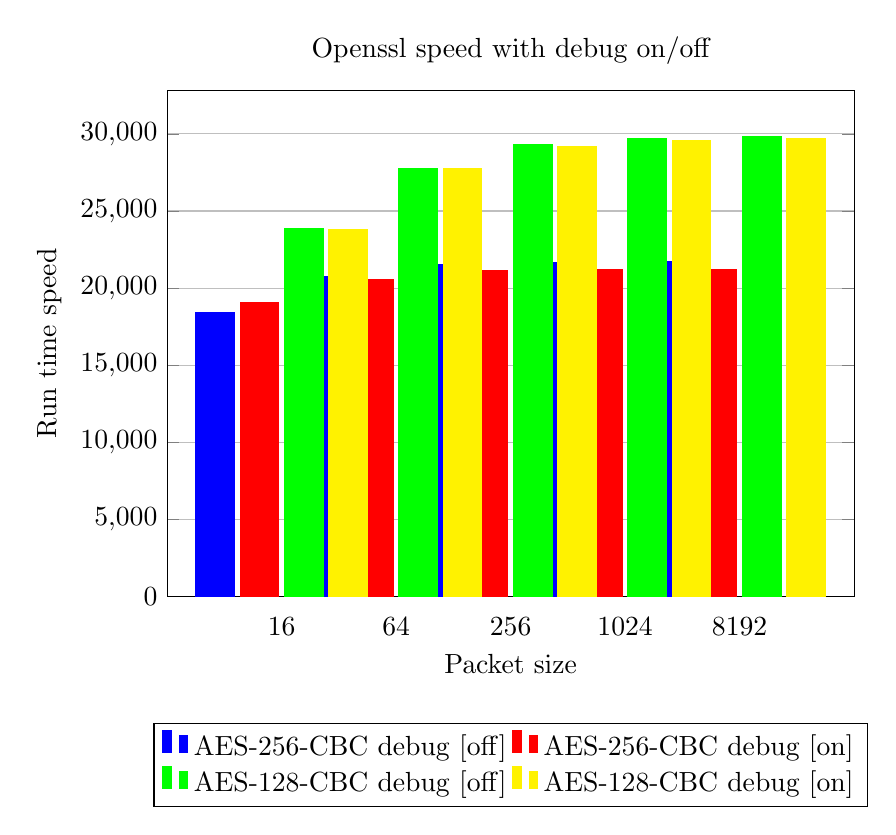
\begin{tikzpicture}
\begin{axis}[
		title = {Openssl speed with debug on/off},
        width  = 0.85*\textwidth,
        height = 8cm,
        major x tick style = transparent,
        ybar,
        bar width=14pt,
        ymajorgrids = true,
        ylabel = {Run time speed},
        xlabel = {Packet size},
        ymin=0,
        symbolic x coords={16,64,256,1024,8192},
        xtick = data,
        scaled y ticks = false,
        legend style={at={(0.5,-0.25)},	anchor=north,legend columns=2},
        enlarge x limits=0.25,
    ]
\addplot[style={blue,fill=blue,mark=none}]
	coordinates {(16,18400.60) (64,20750.61) (256,21507.33) (1024,21681.15) (8192,21725.18)};
	\label{aes-256-cbc-dbg-off}

\addplot[style={red,fill=red,mark=none}]
	coordinates {(16,19091.65) (64,20579.24) (256,21106.60) (1024,21216.26) (8192,21203.63)};
	\label{aes-256-cbc-dbg-on}

\addplot[style={green,fill=green,mark=none}]
	coordinates {(16,23882.41) (64,27781.80) (256,29285.63) (1024,29692.25) (8192,29807.96)};
	\label{aes-128-cbc-dbg-off}

\addplot[style={yellow,fill=yellow,mark=none}]
	coordinates {(16,23806.36) (64,27728.96) (256,29181.70) (1024,29573.46) (8192,29687.81)};
	\label{aes-128-cbc-dbg-on}

\legend{AES-256-CBC debug [off], AES-256-CBC debug [on], AES-128-CBC debug [off], AES-128-CBC debug [on]}
\end{axis}
\end{tikzpicture}

